\chapter{Модельный эксперимент}

\section{Квазиньютоновские методы}

Среди алгоритмов многомерной минимизации следует выделить группу алгоритмов, 
которые объединяют достоинства метода наискорейшего спуска и метода Ньютона. 
Такие алгоритмы принято относить к так называемым квазиньютоновским методам. 
Особенность этих алгоритмов состоит в том, что при их применении нет 
необходимости вычислять и обращать матрицу Гессе целевой функции \( f(x) \) 
и в то же время удается сохранить высокую скорость сходимости алгоритмов, 
присущую методу Ньютона и его модификациям.

\subsection{Общее описание алгоритма}

\newcommand{\grad}{\mathrm{grad}}

Элементы релаксационной последовательности \( \{ x^k \} \) в алгоритмах 
квазиньютоновских методов минимизации непрерывно дифференцируемой в 
\( \mathbb{R}^n \) целевой функции строят \( f(x) \) в соответствии с 
рекуррентным соотношением \( x^k = x^{k-1} + \kappa_k p^k \), но направление 
спуска на каждой \( k \)-й итерации задают в виде
\begin{equation}
    p^k = -A_k \grad f(x^{k-1}) = A_k w^k, k \in \mathbb{N}
    \label{eq:5.23}
\end{equation}

Здесь \( w^k = -\grad f(x^{k-1}) \) -- антиградиент целевой функции в точке 
\( x^{k-1} \), а \( A_k \) -- положительно определенная матрица порядка 
\( n \), обновляемая на \( k \)-й итерации. Отметим, что направление, 
задаваемое на каждой \( k \)-й итерации вектором \eqref{eq:5.23}, \( p^k \) 
является направлением спуска, так как с учетом \eqref{eq:5.23}
\begin{equation}
    \left( \grad f(x^{k-1}, p^k \right) = -\left( w^k, A_k w^k \right) < 0
\end{equation}

Матрица \( \{ A_k \} \) определяют таким образом, чтобы последовательность 
\( \{ A_k \} \) при \( k \leftarrow \infty \) имела предел, равный 
\( H^{-1}(x^*) \), где \( H(x^*) \) -- матрица Гессе целевой функции, 
вычисленная в точке минимума \( x^* \) этой функции. На \( k \)-й итерации 
алгоритма поиска точки минимума происходит спуск из точки \( x^{k-1} \) с 
шагом спуска \( \kappa_k \abs{p^k} \), причем значение \( \kappa_k \) выбирают 
путем исчерпывающего спуска в направлении вектора \( p^k \). На первой 
итерации (\( k = 1 \)) спуск начинают из выбранной начальной точки \( x^0 \) и 
при этом обычно в качестве \( A_1 \) берут единичную матрицу \( I_n \) порядка 
\( n \). 

Если целевая функция является сильно выпуклой, то алгоритмы метода Ньютона 
обладают квадратичной скоростью сходимости. Поэтому можно ожидать, что 
алгоритмы квазиньютоновских методов будут иметь достаточно высокую скорость 
сходимости, если на каждой \( k \)-й итерации матрица \( A_k \) выбрана 
близкой к матрице \( H^{-1}(x^{k-1} \) в точке \( x^{k-1} \in \mathbb{R} \). 
Используя при конструировании матрицы \( A_k \) аппроксимацию матрицы 
\( H^{-1}(x^{k-1} \) с учетом информации о градиенте целевой функции в той же 
точке \( x^{k-1} \) можно существенно упростить процедуру нахождения 
направления спуска на \( k \)-й итерации. Именно эти соображения лежат в 
основе построения алгоритмов квазиньютоновских методов.\cite{bib:methods}

\subsection{Алгоритм Бройдена -- Флетчера -- Гольдфарба -- Шанно}

Среди квазиньютоновских алгоритмов одним из наиболее популярных и используемых 
является так называемый BFGS алгоритм. Также существуют модификация данного 
метода с ограниченным использованием памяти L-BFGS, который предназначен для 
решения нелинейных задач с большим количеством неизвестных, который и 
используется в данной работе.

Данный метод находит минимум любой дважды непрерывно дифференциируемой 
выпуклой функции. Несмотря на эти теоретические ограничения BFGS хорошо 
справляется и с невыпуклыми функциями.

Пусть решается задача оптимизации функционала:
\[ 
    \arg\min_x f(x) 
\]
Методы второго порядка решают данную задачу итерационно, с помощью разложения 
функции в полином второй степени:
\[ 
    f(x_k + p) = f(x_k) + \nabla f^T(x_k) p + \frac{1}{2} p^T H(x_k) p, 
\]
где \( H \) -- гессиан функционала \( f \) в точке \( x \). Зачастую 
вычисление гессиана трудоемки, поэтому BFGS алгоритм вместо настоящего 
значения \( H(x) \) вычисляет приближенное значение \( B_k \), после чего 
находит минимум полученной квадратичной задачи:
\[ 
    p_k = - B_k^{-1}\nabla f(x_k). 
\]
Как правило, после этого осуществляется поиск вдоль данного направления точки, 
для которой выполняются условия Вольфе:
\begin{gather}
    f(x_k + \alpha_k p_k) \leq f(x_k) + c_1 \alpha_k \nabla f_k^T p_k, 
    \nonumber \\
    \nabla f(x_k + \alpha_k p_k)^T p_k \geq c_2 \nabla f_k^T p_k
    \label{eq:wolfe}
\end{gather}

В качестве начального приближения гессиана можно брать любую невырожденную, 
хорошо обусловленную матрицу. Часто берут единичную матрицу. Приближенное 
значение гессиана на следующем шаге вычисляется по формуле:
\[ 
    B_{k + 1} = B_k - \frac{B_k s_k s_k^T B_k}{s_k^T B_k s_k} + 
        \frac{y_k y_k^T}{y_k^T s_k} 
\]
где \( I \) -- единичная матрица, \( s_k = x_{k + 1} - x_k \) -- шаг алгоритма 
на итерации, а изменение градиента на итерации:
\begin{equation} 
    y_k = \nabla f_{k + 1} - \nabla f_{k} 
    \label{eq:y_k}
\end{equation}

Поскольку вычисление обратной матрицы вычислительно сложно, вместо того, 
чтобы вычислять \( B_k \), обновляется обратная \( B_k \) матрица 
\( C_k = B_k^{-1} \):
\begin{equation}
    C_{k + 1} = (I - \rho_k s_k y_k^T)C_k(I - \rho_k y_k s_k^T) + 
        \rho_k s_k s_k^T, 
    \label{eq:c_k}
\end{equation}
где \( \rho_k = ((y^{(k)})^T s^{(k)})^{-1} \).

\clearpage

\begin{algorithm}[H]
    \SetAlgoLined
    \KwData{$x_0, \delta, C_0$}
    $k \gets 0$\;
    \While{ истина }{
        $ d_0 \gets -C_k \nabla f(x_k) $\;
        $ \alpha_k \gets $ Линейный поиск($ x_k, f) $\;
        $ x_{k+1} \gets x_k + \alpha_k d_k $\;
        Посчитать $ C_{k+1} $ из \eqref{eq:c_k}, \eqref{eq:y_k} и
            $ s_k = x_{k+1} - x_k $ \;
        $ k \gets k + 1 $ \;
        \If{$ ||\nabla f(x_k) || \leq \delta $}{
            остановить\;
        }
    }
    \KwResult{$ x_k, f(x_k) $ и $ \nabla f(x_k) $}
    \caption{Алгоритм Бройдена -- Флетчера -- Гольдфарба -- Шанно 
        \cite{skajaa2010limited}}
\end{algorithm}

\section{Метод минимизации энергии}

Функционал свободной энергии ГЛ представленный формулой~\eqref{eq:1}, 
преобразуем к виду
\begin{gather}
    F = \frac{1}{2}\sum\limits_{i=1,2}\left[ 
        \left|\left( \nabla + ie\vec{A}\right)\psi_i\right|^2 + 
        \left( 2\alpha_i + \beta_i |\psi_i|^2 \right)|\psi_i|^2 \right] + 
        \nonumber \\
        \frac{1}{2}\left( \nabla\times\vec{A} \right)^2 - 
        \eta|\psi_1||\psi_2|\cos(\theta_2-\theta_1)
    \label{eqm:1}
\end{gather}

Основные состояния вихревых систем и энергии взаимодействия между вихрями 
находятся с помощью минимизации этого функционала при условии соблюдения 
соответствующих ограничений, таких как расположение вихрей. Для этого разобьём 
рассматриваемую систему на ячейки в виде регулярной сетки. Чтобы иметь 
объективный численный результат используем адаптивно-узловую сетку с шагом 
\( h \) во всей рассматриваемой области. Для того чтобы вычислить энергию 
межвихревого взаимодействия, нужно исправить положение вихрей. Фиксация 
позиции вихря требует особой осторожности, чтобы избежать ситуации, когда 
закрепление на расчетной сетки существенно влияет на вихревое решение. 
Фиксация положения вихря происходит следующим образом. В центре вихря 
плотность равна нулю. Затем фиксируем плотность только доминирующей 
центральной составляющей компоненты \( |\psi_i| \) вихря в данной позиции 
расчетной сетки. Это эффективно предотвращает движения вихря, но не 
препятствует основному расщеплению \( |\psi_1| \) и \( |\psi_2| \) за счет 
магнитного давления. Этот метод <<точки закрепления>> также имеет преимущество 
перед <<малоинвазивным>>, так как только фиксируется положение ядра особенной 
точки. Таким образом этот метод позволяет вычислить средние и 
дальнодействующие силы с наибольшей точностью. Тем не менее, в то же время, 
очевидно, этот способ не работает для слишком малого межвихревого расстояния. 
Малое межвихревое расстояние приводит к следующему легкоузнаваемому артефакту: 
ядро одного из вихрей удлиняется и становится равным нулю на обоих концах 
закрепления, это позволяет убрать второй вихрь из рассмотрения. Такое 
поведение может быть легко исправлено используя различные схемы закрепления, а 
потому, закрепления вихрей на малом расстоянии не имеет отношения к вопросам, 
изучаемых в данной работе, а также для обеспечения согласованности 
используется только одна процедура фиксации.

Сходимость определяется следующим образом:
\begin{enumerate}
    \item Выбирается конкретный шаг сетки \( h_1 \) и число точек сетки 
        \( N_1 = N_{1x} \cdot N_{1y} \) даваемое размером системы
        \( L_x = h \cdot (N_{1x}-1) \), \( L_y = h \cdot (N_{1y}-1) \). 
        Тогда энергия минимизируется пока она не измениться в несколько
        тысячах иттераций. Это даёт \( E(h_1) \).
    \item Уменьшаем шаг сетки \( h \) на коэффициент 2 или 3 при сохранении 
        размера системы \( L_x, L_y \) с помощью сплайн-интерполяции. 
        Затем ещё раз перебираем энергию, пока она не измениться в 
        нескольких тысячах итераций, давая \( E(h_2) \) и так далее. 
        Затем определяем сходимость с помощью формулы
\end{enumerate}
\begin{equation}
    \frac{E(h_n) - E(h_{n+1})}{E(h_n)} = C
\end{equation}

В работе используются сетки размером до \( N \approx 10^7 \) 
(\( L_x = L_y = 1200 \)) что дает очень высокую точность, обычно 
\( C < 10^{-4} \). \cite{bib:minimization}

\section{Задание начальных условий}

Минимизация начинается с начального приближения: конфигурацию поля, несущего
\( N_v \) квантов потока, описываемого
\begin{gather}
    \Phi_a = u_a \prod\limits_{i=1}^{N_\nu} \sqrt{ 
        \frac{1}{2}\left( 1 + \tanh\left( 
            \frac{4}{\xi}\left( \mathcal{R}_i(x,y) - \xi \right)
        \right) \right)
    } e^{i\Theta_i}
    \nonumber \\
    \vec{A} = \frac{1}{e\mathcal{R}}\left( sin\Theta, -\cos\Theta \right)
    \label{eqm:6}
\end{gather}
где \( a = 1,2, u_a \) является вакуумное среднее каждого скалярного поля, 
параметр \( \xi \) даёт размер ядра, а \( \Theta \) и
\( \mathcal{R} \) определяются из
\begin{gather}
    \Theta(x,y) = \sum\limits_{i=1}^{N_v} \Theta_i(x,y), \nonumber \\
    \Theta_i(x,y) = \tan^{-1}\left(\frac{y-y_i}{x-x_i} \right), \nonumber \\
    \mathcal{R}(x,y) = \sum\limits_{i=1}^{N_v} \mathcal{R}_i(x,y), \nonumber \\
    \mathcal{R}_i(x,y) = \sqrt{(x-x_i)^2+(y-y_i)^2}.
\end{gather}
\( (x_i,y_i) \) является начальным положение данного вихря. Тогда, все степени 
свободы находятся в расслабленном состоянии одновременно, без каких-либо 
ограничивающих факторов препятствующих получению точного решения уравнений 
Гинзбурга-Ландау.
\cite{bib:minimization}

\newpage

\section{Результаты модельного эксперимента}

Результаты модельного эксперимента были получены с помощью программы 
представленной в Приложении А. 

Далее идут полученные результаты модельного эксперимента, при различных 
параметрах, уравнения Гинзбурга-Ландау \eqref{eq:2} для вихрей абрикосова в 
сверхпроводнике полуторного рода.

\begin{table}[h!]
    \centering
    \begin{tabular}{|c|c|}
        \hline 
        Параметр & Значение \\ \hline
        \( N_x, N_y \) & \( 1200 \) \\ \hline
        \( \alpha_{1,2} \) & \( (-1.0, -0.0625) \) \\ \hline
        \( \beta_{1,2} \) & \( (1.0, 0.25) \) \\ \hline
        \( \eta \) & \( 0.3 \) \\ \hline
        \( e \) & \( 0.7 \) \\ \hline
    \end{tabular}
    \caption{Параметры ГЛ используемые для модельного эксперимента №1.}
    \label{param:01}
\end{table}

\begin{figure}[h!]
    \center
    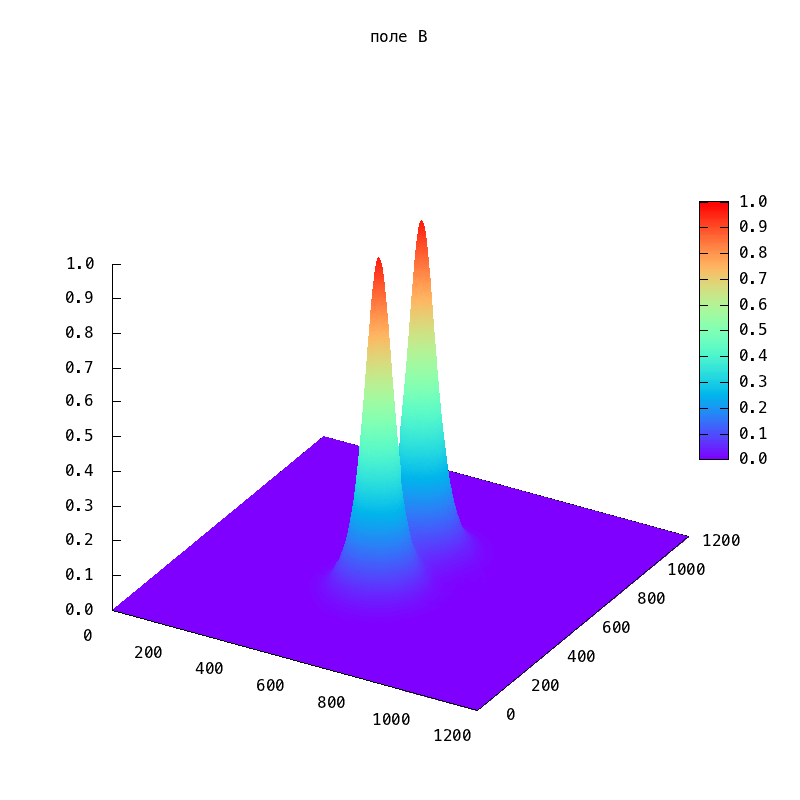
\includegraphics[width=0.8\textwidth]{data_01/3d_B}
    \caption{Распределение магнитного поля для вихрей абрикосова в 
        сверхпроводнике 1,5-го рода при параметрах из Таблицы \ref{param:01}.}
    \label{img:3d-field-B-01}
\end{figure}

\begin{figure}[h!]
    \center
    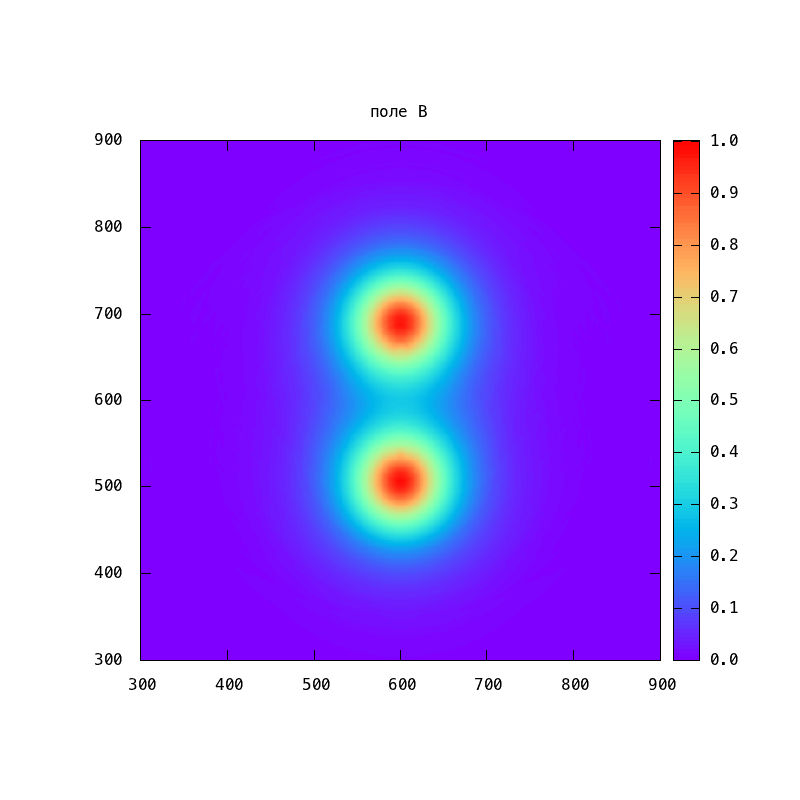
\includegraphics[width=0.8\textwidth]{data_01/map_B}
    \caption{Вид линий уровня Рисунка \ref{img:3d-field-B-01}. 
        Рассматриваемая область увеличена.}
    \label{img:map-field-B-01}
\end{figure}

\begin{figure}[h!]
    \center
    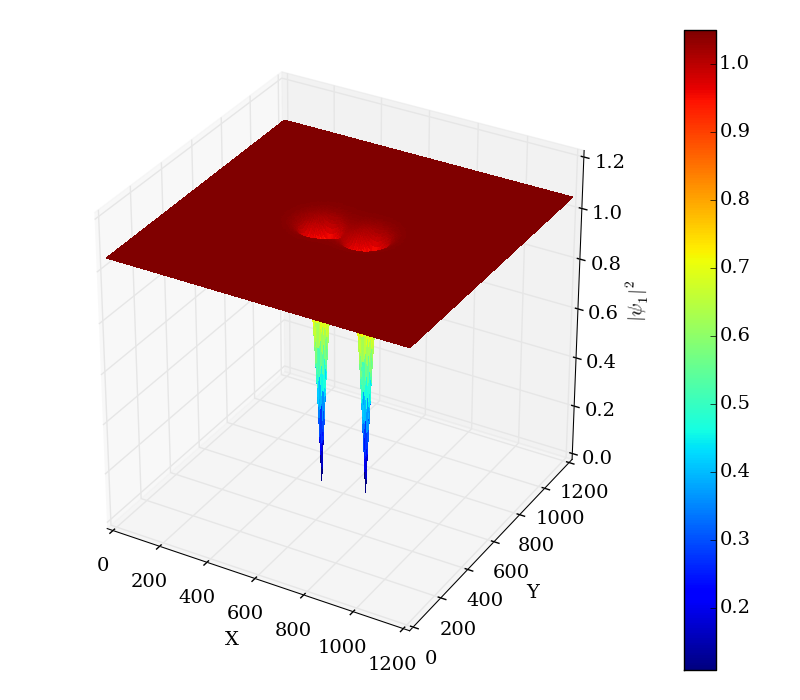
\includegraphics[width=0.8\textwidth]{data_01/3d_F1}
    \caption{Характерный вид энергии взаимодействия первой зоны в 
        сверхпроводнике (\( \abs{\psi_1}^2 \)-компонента).}
    \label{img:3d-band-1-01}
\end{figure}

\begin{figure}[h!]
    \center
    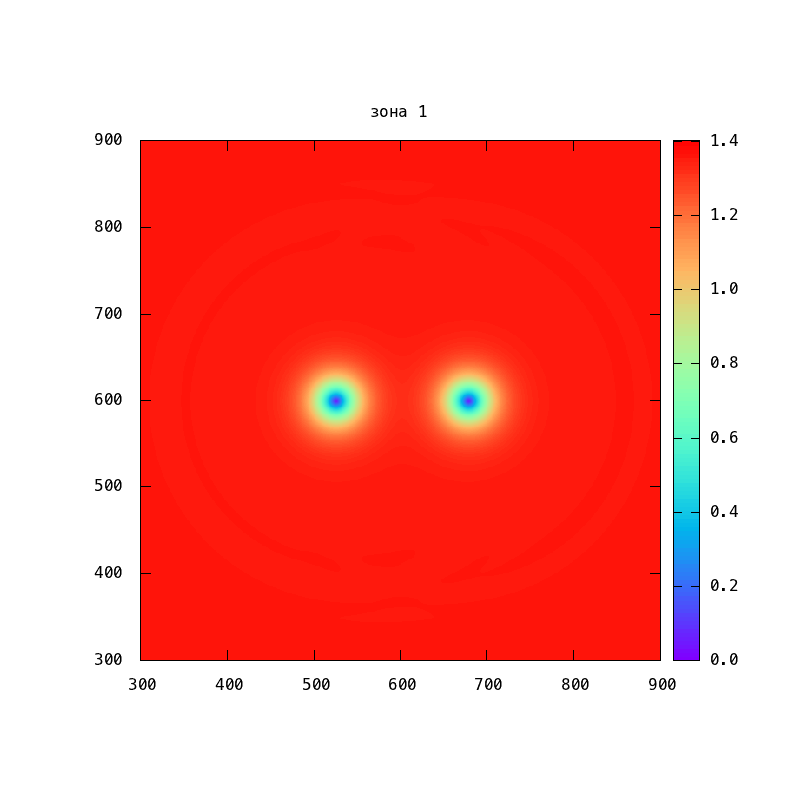
\includegraphics[width=0.8\textwidth]{data_01/map_F1}
    \caption{Вид линий уровня Рисунка \ref{img:3d-band-1-01}. 
        Рассматриваемая область увеличена.}
    \label{img:map-band-1-01}
\end{figure}

\begin{figure}[h!]
    \center
    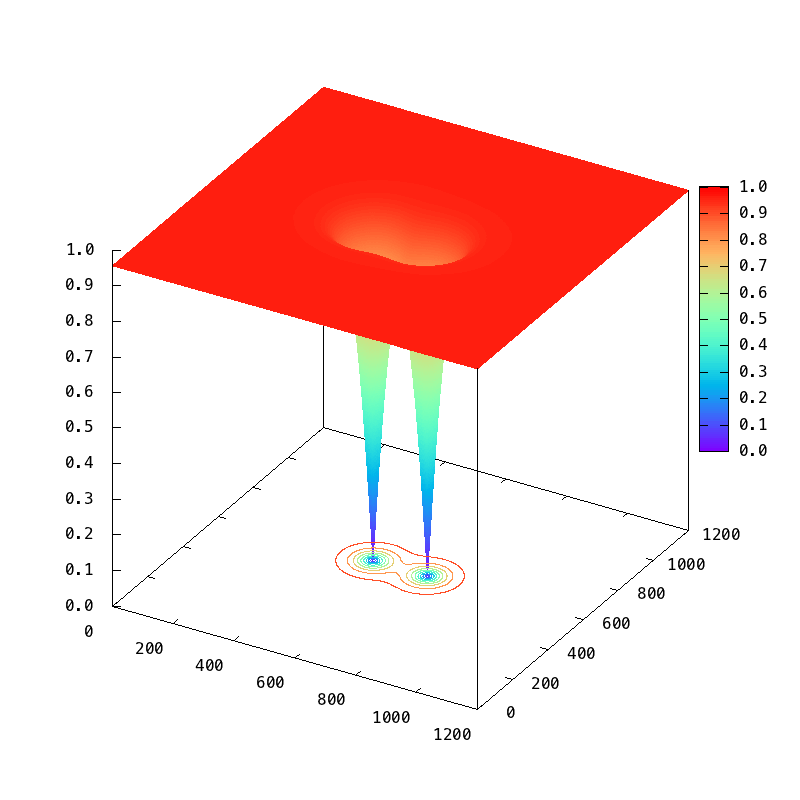
\includegraphics[width=0.8\textwidth]{data_01/3d_F2}
    \caption{Характерный вид энергии взаимодействия первой зоны в 
        сверхпроводнике (\( \abs{\psi_2}^2 \)-компонента).}
    \label{img:3d-band-2-01}
\end{figure}

\begin{figure}[h!]
    \center
    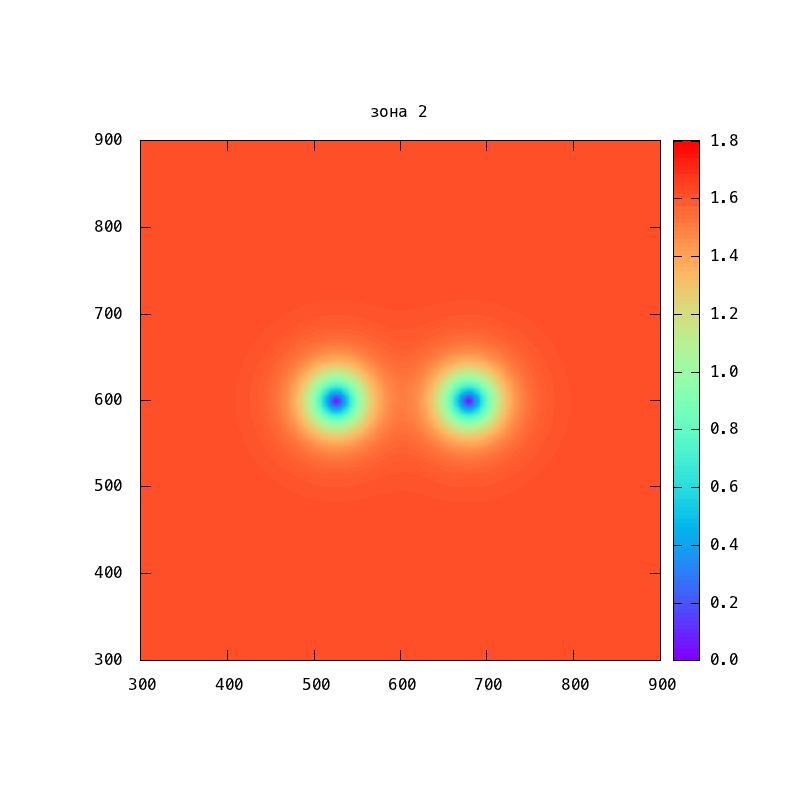
\includegraphics[width=0.8\textwidth]{data_01/map_F2}
    \caption{Вид линий уровня Рисунка \ref{img:3d-band-2-01}. 
        Рассматриваемая область увеличена.}
    \label{img:map-band-2-01}
\end{figure}

\begin{figure}[h!]
    \center
    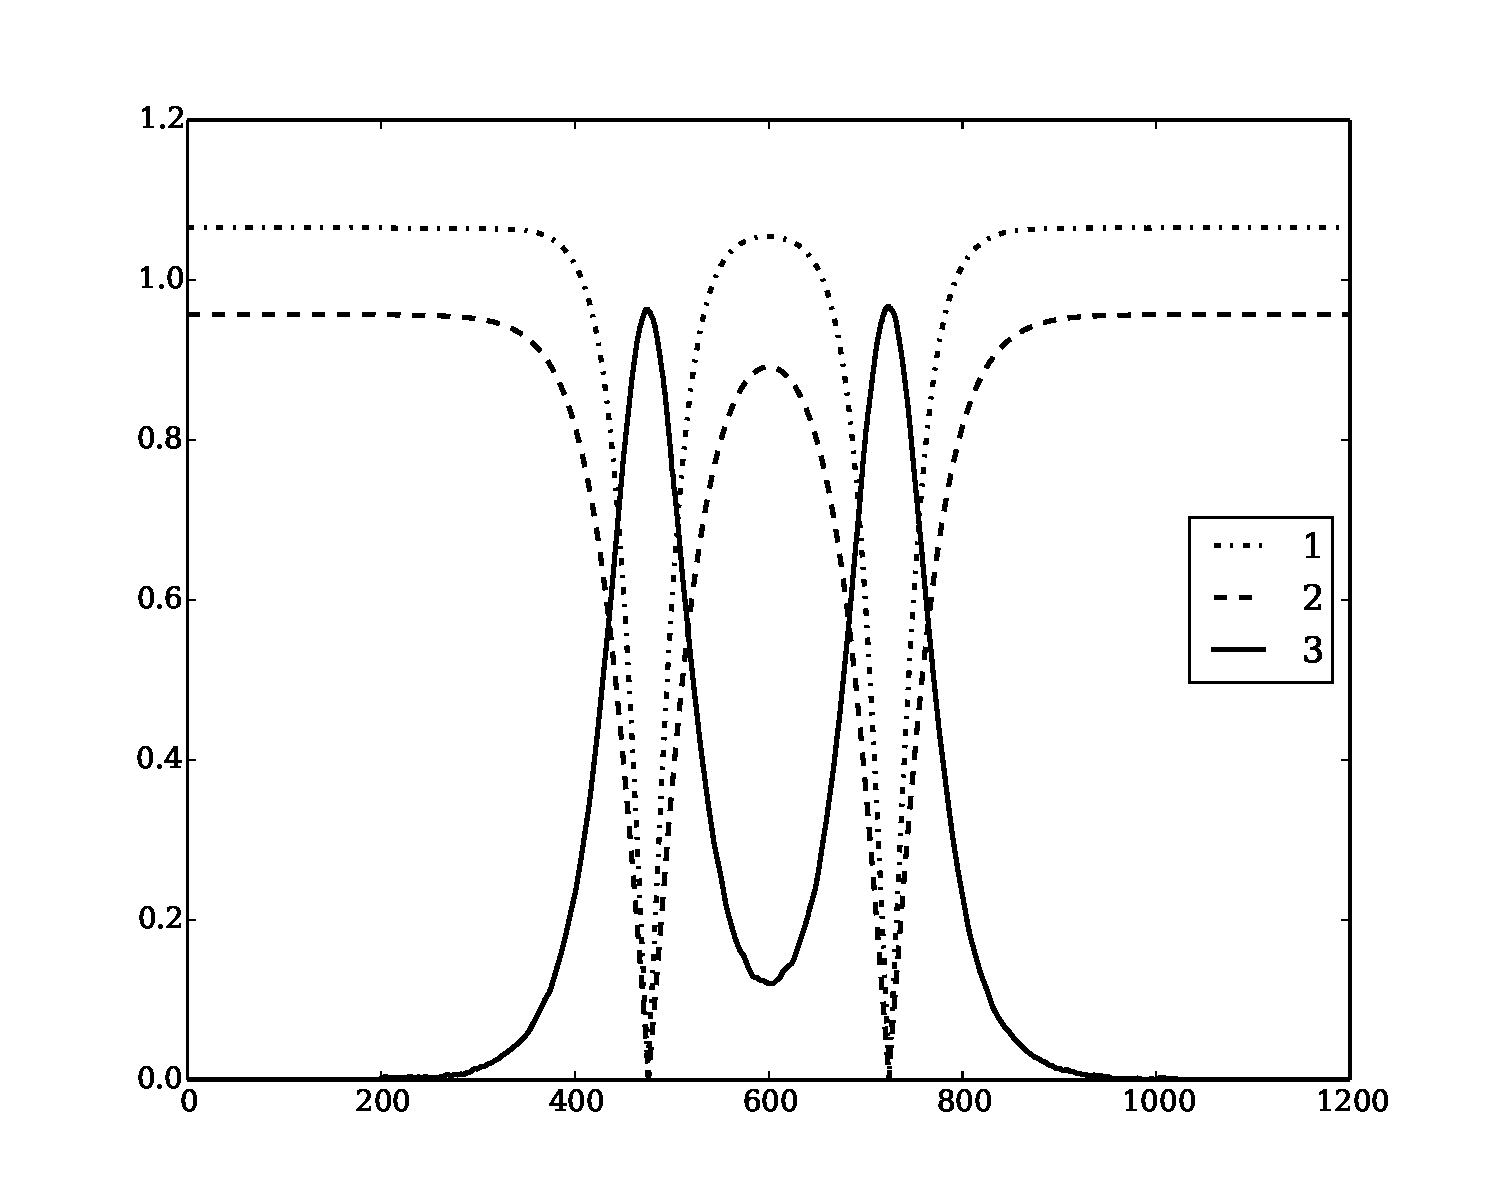
\includegraphics[width=0.8\textwidth]{data_01/band_profile}
    \caption{График поперечного сечения, показывающий форму вихря, полученный 
        для двух взаимодействующих абрикосовских вихрей в сверхпроводнике 
        полуторного рода. Здесь \( 1 \) -- первая активная зона в 
        сверхпроводнике (\( \abs{\psi_1}^2 \)-компонента), \( 2 \) -- вторая 
        (\( \abs{\psi_2}^2 \)-компонента), а \( 3 \) -- распределение 
        магнитного поля в системе (\( B \)-компонента).}
    \label{img:band-profile-01}
\end{figure}

\newpage